%Общий объем раздела 20-30 стр. (16 are done)

\section{Анализ предметной области. Обзор известных работ в области классического стегоанализа}

\subsection{Базовые понятия и положения стеганографии}

\textit{Стеганография} (от греч. στεγανός — скрытый и γράφω — пишу; буквально «тайнопись») — это наука о передаче (хранении) информации с сохранением в тайне самого факта передачи (хранения). Большинство способов классической цифровой стеганографии базируется на особенностях восприятия информации человеком, организуя сокрытие секретных сообщений таким образом, что чувствительность человеческих органов не позволяет определить их наличие.

Основными понятиями стеганографии являются понятия контейнера, сообщения и ключа. Ниже приведены их определения, данные в монографии~\cite{Agranovskiy}.

\textit{Контейнером} $ b $ ($ b \in \mathbb{B} $, где $ \mathbb{B} $ — множество всех возможных контейнеров) называют несекретные данные, используемые для сокрытия сообщений. В цифровой стеганографии роль контейнеров играют растровые графические изображения, цифровой звук, а также текстовые и другие электронные документы.

\textit{Сообщением} $ m $ ($ m \in \mathbb{M} $, где $ \mathbb{M} $ — множество всех возможных сообщений) называют секретную информацию, скрываемую в контейнере.

\textit{Ключом} $ k $ ($ k \in \mathbb{K} $, где $ \mathbb{K} $ — множество всех возможных секретных ключей) называют секретную информацию, известную только санкционированному пользователю стеганосистемы, которая определяет конкретный способ сокрытия и извлечения сообщения. В широком смысле ключ — это неизвестный противнику способ (алгоритм) сокрытия информации, в узком — параметр заранее оговорённого стеганографического алгоритма, без знания которого извлечение сообщения невозможно.

\textit{Пустой контейнер} --- это некоторый контейнер $ b $, не содержащий какого-либо сообщения $ m $.

\textit{Заполненный контейнер} --- это контейнер $ b $, содержащий сообщение $ m $.

Помимо приведённых определений распространены следующие термины.

\textit{Стеганографическая система (стегосистема)} --- совокупность средств, осуществляющих встраивание сообщения в контейнер и его последующее извлечение.

\textit{Пропускная способность стегосистемы} $ C $~--- отношение максимально возможного объёма встроенного сообщения к объёму контейнера при сохранении необходимого уровня стегоустойчивости.

\textit{Стегоустойчивость} --- свойство стегосистемы, характеризующее её способность обеспечивать заданное качество стегосвязи в условиях наличия различных деструктивных факторов (шумы, атаки противодействия передаче сообщения).

\textit{Стегоскрытность} --- свойство стегосистемы, характеризующее её способность обеспечивать невозможность факта наличия стегосвязи.

Общая схема стеганографической системы приведена на рис. 1.1. Согласно ей, на передающей стороне сообщение скрывается в контейнере при помощи прямого стеганографического преобразования. Затем полученный заполненный контейнер по открытому каналу связи отправляется принимающей стороне, где при помощи обратного стеганографического преобразования извлекается исходное сообщение.

\begin{figure}
\centering
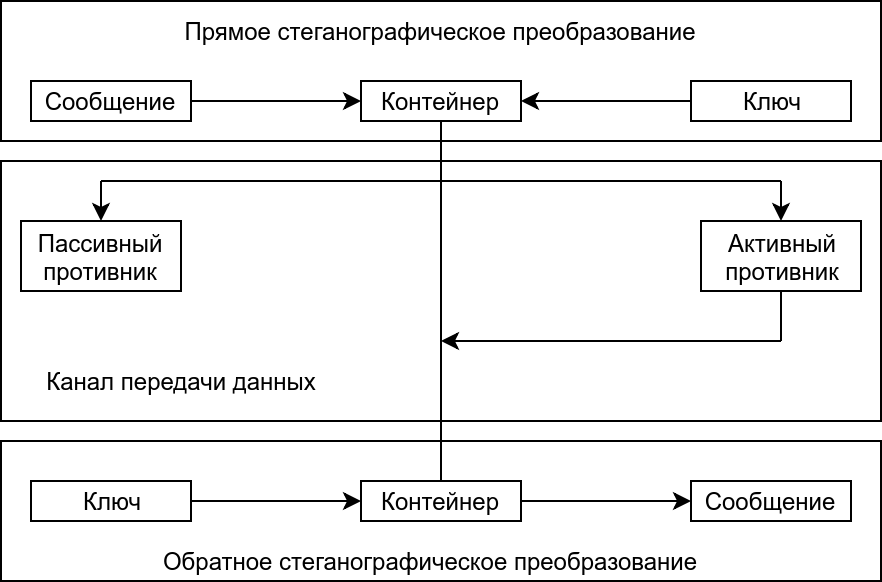
\includegraphics[width=1\textwidth]{include/graphics/stego_system_scheme}
\caption{Обобщённая схема стеганографической системы}
\label{fig:StegoSystem}
\end{figure}

Задача \textit{пассивного противника} состоит в определении факта наличия в контейнере сокрытых данных (атака детектирования). \textit{Активный противник} пытается вносить изменения в контейнер или, в простейшем случае, уничтожить передаваемое сообщение (атака уничтожения данных).

\subsection{Метод замены наименее значимого бита} \label{sec:LSB}

Наиболее распространённым и примитивным методом сокрытия данных в пространственной области изображений является метод замены наименее значимого бита (англ. Least Significant Bit replacing; также метод замены НЗБ). Одним из его основных преимуществ является низкая вычислительная сложность, основным недостатком --- низкая устойчивость к атакам детектирования и уничтожения данных.

Обозначим пустой стегоконтейнер в оттенках серого размера $ {n_1 \times n_2} $ как $ X = (x_{ij}) \in \mathbb{Q} = \{0, \dotsc, 255\}^{n_1 \times n_2} $, а соответствующий заполненный контейнер как $ Y = (y_{ij}) \in \mathbb{Q} $.

Младший бит пикселя изображения в оттенках серого хранит младший разряд соответствующего двоичного числа и, следовательно, его изменение минимально влияет на изменение числа в целом. Отсюда следует, что встраивание произвольной битовой последовательности в младшие биты пикселей повлечёт за собой минимальной визуальное искажение стегоконтейнера. К тому же, такая методика встраивания обеспечивает довольно высокую пропускную способность $ C = 1 $ бит/пиксель.

Пустой контейнер можно представить в двоичной форме следующим образом:

\begin{equation*}
(x_{ij}) = \sum_{p = 0}^8 (x_{ij})_p \cdot 2^p.
\end{equation*}

Тогда заполненный стегоконтейнер имеет вид:

\begin{equation*}
(y_{ij}) = \sum_{p = 1}^8 (x_{ij})_p \cdot 2^p + m_{ij},
\end{equation*}
где $ m_{ij} \in {0, 1} $ --- бит стегосообщения, имеющего вид матрицы размера $ {n_1 \times n_2} $.

Существует множество нетривиальных модификаций данного метода. Интересным для рассмотрения примером является алгоритм, описанный в~\cite{FridrichLossless}. Он предназначен для стеговстраивания цифровых водяных знаков. В таком случае контейнер является не только средой передачи сообщения, которую можно выбрать для обеспечения необходимого уровня скрытности и пропускной способности относительно конкретного сообщения, но и несёт собственную ценность, что повышает требования к уровню искажений, вносимых при стеговстраивании. К тому же, в некоторых областях применения (например, в медицинской отрасли) наличие искажений, приемлемых для передачи сообщений, недопустимо. Рассматриваемый метод учитывает это и обеспечивает обратимость внесения искажений.

Первым шагом операции встраивания является разделение пикселей $ (x_{ij}) $ на непересекающиеся группы из $ n $ пикселей $ G = (x_1, x_2, \ldots, x_n) $. Для примера выбираются группы из $ n = 4 $ последовательных пикселей в строке. Затем определяется различающая функция $ f(x_1, x_2, \ldots, x_n) \in \mathbb{R} $, имеющая следующий вид:
\begin{equation*}
f(x_1, x_2, \ldots, x_n) = \sum_{i = 1}^{n - 1} \lvert x_{i + 1} - x_i \rvert.
\end{equation*}

Назначением данной функции является оценка гладкости или «регулярности» группы пикселей~$ G $.

Следующим этапом является применение обратимой операции сдвига $ F $, модифицирующей яркость пикселя на близкое значение. Например, операцию $ F $, меняющую НЗБ, можно определить следующим образом: $ 0 \leftrightarrow 1, 2 \leftrightarrow 3, \ldots, 254 \leftrightarrow 255 $. Обозначим данную операцию $ F_1 $. Тогда $ F_{-1} $ применяется по следующей схеме: $ -1 \leftrightarrow 0, 1 \leftrightarrow 2, 3 \leftrightarrow 4, \ldots, 253 \leftrightarrow 254, 255 \leftrightarrow 256 $. Для полноты введём $ F_0(x) = x \quad \forall x \in \mathbb{Q} $.

Различающая функция $ f $ и операция сдвига $ F $ применяются для классификации групп пикселей~$ G $:
\begin{equation}
\begin{cases}
G \in \mathbb{R} \Longleftrightarrow f(F(G)) > f(G), \\
G \in \mathbb{S} \Longleftrightarrow f(F(G)) < f(G), \\
G \in \mathbb{U} \Longleftrightarrow f(F(G)) = f(G).
\end{cases}
\label{RulesForGroups}
\end{equation}

Группы, принадлежащие ко множествам $ \mathbb{R} $, $ \mathbb{S} $ и $ \mathbb{U} $ называются регулярными, сингулярными и неиспользуемыми соответственно. $ N_R $, $ N_S $ и $ N_U $ --- количество упомянутых групп в изображении.

Из~\ref{RulesForGroups} видно, что:
\begin{equation*}
\begin{cases}
\forall G \in \mathbb{R} \quad F(G) \in S, \\
\forall G \in \mathbb{S} \quad F(G) \in R, \\
\forall G \in \mathbb{U} \quad F(G) \in U.
\end{cases}
\end{equation*}

Таким образом, возможно ввести соответствие между $ G \in \mathbb{R} $ и единичным битом встраиваемого сообщения и $ G \in \mathbb{S} $ и нулевым битом, применяя $ F $ в случае несоответствия типа группы очередному биту сообщения. Для восстановления оригинального изображения предлагается составить карту принадлежности всех $ G $ изображения множествам и разместить её в начале встраиваемого сообщения.

Пропускная способность данного метода $ C = N_R + N_S = {n_1}{n_2}/{n} - N_U $. Количество неиспользуемых групп напрямую влияет на пропускную способность, что существенно ограничивает длину сообщения при встраивании в астрономические снимки и другие изображения с продолжительными участками пикселей равной яркости. Для устранения этого недостатка предлагается использовать различные операторы сдвига $ F $ для пикселей группы $ G $, а для записи соответствия между оператором и пикселем --- маску $ M $, представляющую собой последовательность из $ n $ чисел, принимающих значения $ -1 $, $ 0 $ и $ 1 $. Тогда $ F_M(G) = (F_{M(1)}(x_1), F_{M(2)}(x_2), \ldots, F_{M(n)}(x_n)) $.

\subsection{Основные принципы и подходы стегоанализа}

\textit{Стегоанализ} — это наука о выявлении факта передачи скрытой информации в анализируемых данных, её извлечении или уничтожении.

В зависимости от наличия априорных знаний о стегосистеме, задействованной при стеговстраивании, применяются направленные или слепые методы стегоанализа. \textit{Направленные} методы стегоанализа предназначены для выявления присутствия сообщения, вложенного известным стегоаналитику методом. В случае отсутствия данных о стегоалгоритме встраивания используют методы \textit{слепого} стегоанализа.

Следующий критерий классификации стегоаналитических методов --- используемый подход. В зависимости от подхода можно выделить \textit{визуальные}, \textit{сигнатурные}, \textit{схемные} и \textit{статистические} методы. Рассмотрим их применительно к стегоанализу цифровых неподвижных изображений.

\textbf{Визуальные методы} основаны на способностях зрительной системы человека, а именно, возможности анализировать зрительные образы и определять различия в сопоставляемых изображениях.

Такие методы стегоанализа графических файлов являются самыми простыми в реализации, но они неспособны обнаружить сообщения, встроенные с помощью современных методов стеговстраивания, и подвержены влиянию человеческого фактора в лице оператора-аналитика.

Подходом \textbf{сигнатурных методов} является синтаксический анализ последовательности битов анализируемого контейнера.

В первых известных алгоритмах сокрытия сообщений в цифровых изображениях заполнение контейнера производилось путём замены служебных атрибутов файла на встраиваемую информацию~\cite{FridrichBook}, что позволяло относительно просто составить сигнатуру, характеризующую заполненный стегоконтейнер, и свести задачу стегоанализа к задаче поиска сигнатуры.

Дальнейшее усовершенствование стеганографических методов привело к широкому распространению стегосистем, осуществляющих встраивание в пространственной области изображения, но сигнатурные методы всё ещё могли противостоять таким стегосистемам. Например, в работе~\cite{HideAndSeek} описывается сигнатурный метод стегоанализа изображений в оттенках серого, стеганографически заполненных с помощью программы Hide and Seek версий 4.1 и 5.0. Заполненный контейнер представляет собой изображение, содержащее три канала цветности (цветовая модель RGB) с одинаковыми значениями яркости в каждом. Наиболее распространённым способом хранения трёхканальных изображений является кодирование каждой цветовой координаты пикселя 8-битным числом, определяющим диапазон уровней квантования $ \mathbb{Q} = \{0, \dotsc,255\} $ и шаг квантования $ h = 1 $. Hide and Seek использует $ \mathbb{Q} = \{0, \dotsc,252\} $ и $ h = 4 $, что позволяет выделить контейнеры, заполненные этой программой, на общем фоне благодаря меньшему количеству градаций яркости и отсутствию абсолютно белого цвета. Столь грубый подход также приводит к высокой визуальной заметности стеганографического искажения, вплоть до очевидного повреждения изображения~(рис.~\ref{fig:HideAndSeek}).

\begin{figure}
     \centering
     \hspace*{\fill}%
     \begin{subfigure}[b]{0.3\textwidth}
         \centering
         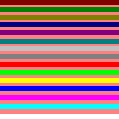
\includegraphics[width=\textwidth]{include/graphics/hide_and_seek_before}
     \end{subfigure}
     \hfill
     \begin{subfigure}[b]{0.3\textwidth}
         \centering
         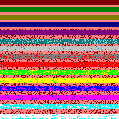
\includegraphics[width=\textwidth]{include/graphics/hide_and_seek_after}
%         \caption{$y=3sinx$}
         %\label{fig:three sin x}
     \end{subfigure}
     \hspace*{\fill}%
     \caption{Пустой и заполненный в Hide and Seek контейнеры}
     \label{fig:HideAndSeek}
\end{figure}

Преимуществом данного подхода является высокая скорость работы реализующих его алгоритмов, но сильная привязка к атрибутам заполненных стегоконтейнеров, не учитывающая принципы стеговстраивания, является существенным недостатком, не позволяющим широко использовать данный подход.

\textbf{Схемные методы} применяются для проверки гипотез о наличии стеганографического встраивания с применением известной стегосистемы.

Основными достоинствами схемных методов являются низкая вероятность возникновения ошибок и возможность идентификации стеганографической системы с последующим извлечением сообщения.

Фатальными недостатками данного подхода являются невозможность реализовать необходимое для применения слепого стегоанализа количество стегосистем и многообразие ключей, позволяющее стегосистеме менять характер стеговстраивания от одного ключа к другому.

\textbf{Статистические методы} базируются на понятии «естественного» контейнера. Их суть заключается в оценивании вероятности существования стегосообщения, встроенного неизвестной стегосистемой на основе критерия близости исследуемого контейнера к «естественному» путём обнаружении отклонения анализируемой информации от ожидаемой модели.

Преимуществом подхода является возможность применения в слепом стегоанализе, недостатком — высокая сложность создания модели «естественного» контейнера.

\subsection{Известные методы стегоанализа на основе статистической обработки данных}

\subsubsection{Метод анализа гистограмм}

Метод анализа гистограмм применяется при наличии гипотезы о распределении элементов пустого контейнера $ (x_{ij}) $. Для анализируемого контейнера $ (b_{ij}) $, о заполненности которого нет априорного знания, строят такую же гистограмму. По отклонению распределения, полученного для $ (b_{ij}) $, от распределения, характерного для $ (x_{ij}) $, судят о заполненности $ (b_{ij}) $. Примером атаки на стегосистему, использующую метод замены наименее значимого бита, может служить построение гистограммы яркости пикселей. Рис.~\ref{fig:LSBHists} наглядно иллюстрирует эффект группировки различных значений яркости, вызванный заменой НЗБ и выражающейся в ступенчатом характере гистограммы.

\begin{figure}
     \centering
     \begin{subfigure}{\textwidth}
         \centering
         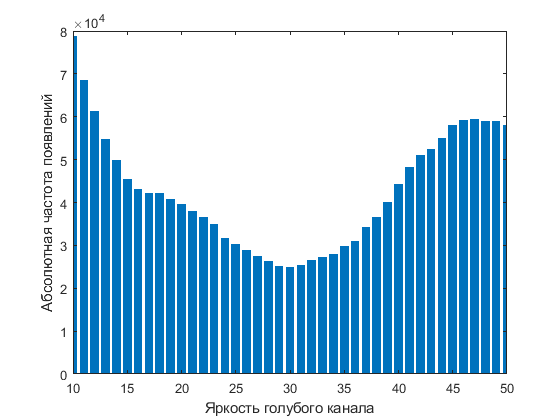
\includegraphics[width=\textwidth]{include/graphics/lsb_subst_before}
     \end{subfigure}
     \hfill
     \begin{subfigure}{\textwidth}
         \centering
         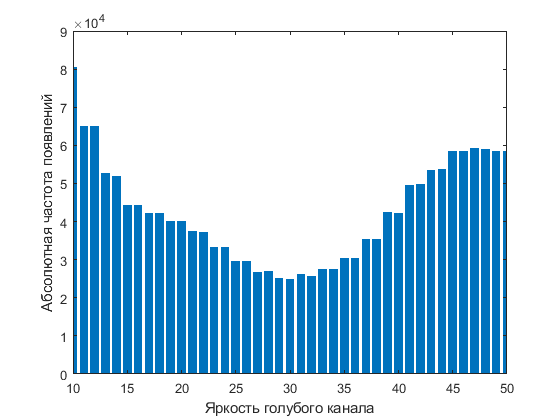
\includegraphics[width=\textwidth]{include/graphics/lsb_subst_after}
     \end{subfigure}
     \caption{Гистограммы до и после применения метода замены НЗБ}
     \label{fig:LSBHists}
\end{figure}

Данный метод также используется для анализа частоты появления серий $ k $ наименее значимых битов значений яркости пикселей. Для построения гистограммы подсчитывается частота равенства последнего НЗБ нулю и единице ($ k = 1 $), двух НЗБ сериям-двойкам ($ 00 $, $ 01 $, $ 10 $, $ 11 $; $ k = 2 $), трёх НЗБ сериям-тройкам ($ 000 $, $ 001 $, $ 010 $, $ 011 $, $ 100 $, $ 101 $, $ 110 $, $ 111 $; $ k = 3 $) и т. д. Для заполненных контейнеров характерна близость частот, в пустых данная симметрия не наблюдается.

\subsubsection {RS-анализ}

RS-анализ был предложен в~\cite{FridrichRSAnalysis} и основывается на модификации метода замены НЗБ, описанного в разделе~\ref{sec:LSB}.

Введём обозначение $ R_M $ для относительного количества регулярных групп с маской $ M $ среди всех групп изображения. Аналогично, обозначим относительное количество сингулярных групп $ S_M $. Тогда $ R_M + S_M \leq 1$ и $ R_{-M} + S_{-M} \leq 1$ для обратной маски. Статистическая гипотеза данного стегоаналитического метода утверждает, что для пустого контейнера
\begin{equation}
\label{eq:RSAnalysisHypothesis}
\begin{cases}
R_M \approx R_{-M}, \\
S_M \approx S_{-M}.
\end{cases}
\end{equation}

Экспериментально выяснено, что для изображений с рандомизированными НЗБ пикселей равенства~\ref{eq:RSAnalysisHypothesis} не соблюдаются. Это наглядно иллюстрирует рис.~\ref{fig:RSDiagram}.

\begin{figure}[h]
     \centering
     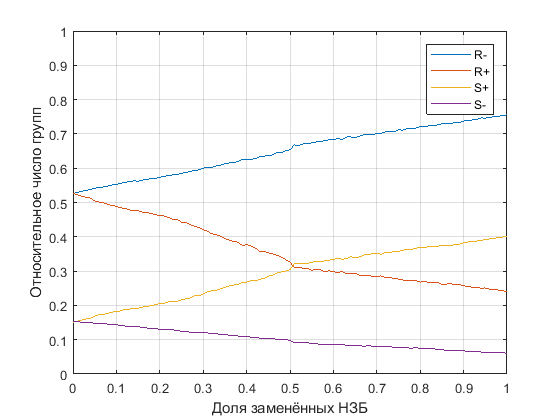
\includegraphics[width=1\textwidth]{include/graphics/rs_diagram}
     \caption{Пример RS-диаграммы}
     \label{fig:RSDiagram}
\end{figure}

RS-диаграмма представляет собой график зависимости относительного числа групп различного типа от доли заменённых НЗБ. Диаграмма, изображённая на рис.~\ref{fig:RSDiagram} показывает, что пары $ R_M $ --- $ R_{-M} $ и $ S_M $ --- $ S_{-M} $ действительно очень близки для пустых контейнеров. Также видно, что разница между $ R_M $  и $ S_M $ стремится к нулю при увеличении длины $ p $ сообщения $ m $, пока оно не заполнит 50~\% пикселей. Для $ R_{-M} $ и $ S_{-M} $ можно наблюдать обратный эффект: разница между ними растёт с увеличением $ p $.

Принцип данного стегоаналитического метода заключается в построении RS-диаграммы и поиске точек пересечения пар кривых путём решения уравнения
\begin{equation*}
2(d_1 + d_0)x^2 + (d_{-0} - d_{-1} - d_1 - 3{d_0})x + d_0 - d_{-0} = 0,
\end{equation*}
где
\begin{equation*}
\begin{cases}
d_0 = R_M(p/2), - S_M(p/2), \\
d_{-0} = R_{-M}(p/2), - S_{-M}(p/2), \\
d_1 = R_M(1 - p/2), - S_M(1 - p/2), \\
d_{-1} = R_{-M}(1 - p/2), - S_{-M}(1 - p/2). \\
\end{cases}
\end{equation*}

Корень уравнения $ x $ позволяет найти $ p $:
\begin{equation*}
p = x/(x - 1/2).
\end{equation*}

\subsection{Применение машины опорных векторов в задачах стегоанализа}

Стегоаналитические методы, использующие машинное обучение, занимают особую нишу: они предоставляют мощный инструментарий для построения слепых стегоаналитических систем, способных детектировать множество стеганографических методов вне зависимости от области встраивания. Ещё одним существенным преимуществом данной группы методов в сравнении с традиционными практиками стегоанализа является возможность учёта более сложных статистических зависимостей между элементами контейнеров, обеспечиваемая агрегированием большого количества характеристик контейнера.

Рассмотрим процедуру обучения с учителем: на вход обучаемой системы подаётся набор тренировочных примеров, который обычно называют\textit{обучающим} или \textit{тренировочным набором данных}, состоящих из пар «стимул --- реакция». Задача стегоаналитической системы состоит в том, чтобы дополнить стимулы из \textit{тестового набора данных}, не участвовавшего в обучении, соответствующими реакциями. Работоспособность подхода обеспечивается подобностью данных, доступных для обучения, и данных, на которых впоследствии применяется обученная модель.

Задачи обучения с учителем обычно делятся на задачи \textit{классификации} и \textit{регрессии}. В задаче классификации поданный на вход объект соотносится с одним из классов, в задаче регрессии требуется предсказать значение некоей функции, у которой обычно может быть бесконечно много разных решений.

Применительно к классификации пары «стимул --- реакция» можно интерпретировать как пары «объект --- класс объекта». В качестве объектов могут выступать контейнеры либо \textit{признаки} --- заранее выбранные характеристики объектов, позволяющие судить об их принадлежности к тому или иному классу.

Машина опорных векторов (МОВ; англ. SVM, support vector machine) --- набор алгоритмов обучения с учителем, использующихся для классификации. Различают три основных типа МОВ:
\begin{enumerate}
\item линейная сеперабельная МОВ;
\item линейная несеперабельная МОВ;
\item нелинейная МОВ.
\end{enumerate}

Рассмотрим задачу обучения по прецедентам $ \langle X, Y, y^*, X^l \rangle $, где $ X $~--- пространство объектов, $ Y $~--- множество ответов, $ y^*: X \to Y $~--- целевая зависимость, значения которой известны на объектах обучающей выборки $ X^l = (x_i, y_i)_{i = 1}^l $, $ y_i = y^*(x_i) $. Алгоритм $ a: X \to Y $ аппроксимирует целевую зависимость $ y^* $ на всём пространстве $ X $.

Для задачи классификации на два непересекающихся класса, в котором объекты описываются $ n $\=/мерными вещественными векторами, $ X = \mathbb{R}^n $, $ Y = \{-1, +1\} $. Алгоритм линейного порогового классификатора имеет вид:
\begin{equation*}
a(x) = sign(\sum_{j = 1}^n w_j x^j - w_0) = sign(\langle w, x \rangle - w_0),
\end{equation*}
где $ x = (x^1, \ldots, x^n) $~--- признаковое описание объекта $ x $; вектор $ w = (w^1, \ldots, w^n) \in \mathbb{R}^n $ и скалярный порог $ w_0 \in \mathbb{R} $ являются параметрами алгоритма.

Уравнение $ \langle w, x \rangle = w_0 $ описывает гиперплоскость размерности $ n - 1 $, разделяющую классы в пространстве $ \mathbb{R}^n $.

Предположим, что выборка разделима, то есть существуют такие значения параметров $ w, w_0 $, при которых функционал числа ошибок
\begin{equation*}
Q(w, w_0) = \sum_{i = 1}^l [y_i(\langle w, x_i \rangle - w_0) < 0]
\end{equation*}
принимает нулевое значение. Тогда разделяющая гиперплоскость не единственна: существуют другие её положения, реализующие то же самое разбиение выборки. Для достижения наименьшего значения $ Q(w, w_0) $ МОВ накладывает на разделяющую гиперплоскость требование соблюдения максимальной дистанции от ближайших к ней точек обоих классов. Таким образом, задаётся полоса, разделяющая классы, в которой не лежат точки обучающей выборки. Границами полосы служат две параллельные гиперплоскости, на которых лежат точки, ближайшие к разделяющей гиперплоскости. При этом сама разделяющая гиперплоскость проходит ровно по середине полосы.

В общем случае гарантировать линейную разделимость выборки не представляется возможным, поэтому на практике используют линейный несеперабельный МОВ, позволяющий алгоритму допускать ошибки и стремящийся к минимизации их количества.

Существует ещё один подход к решению проблемы линейной неразделимости --- переход от исходного пространства признаковых описаний объектов $ X $ к новому пространству $ H $ с помощью некоторого преобразования $ \psi: X \to H $. Если пространство имеет достаточно высокую размерность, то можно надеяться, что в нём выборка окажется линейно разделимой (если выборка $ X^l $ не противоречива, то всегда найдётся пространство размерности не более $ l $, в котором выборка будет линейно разделима). Пространство $ H $ называют \textit{спрямляющим}. Пример результата обучения нелинейной МОВ приведён на~\ref{fig:NonLinSVM}.

\begin{figure}[h]
     \centering
     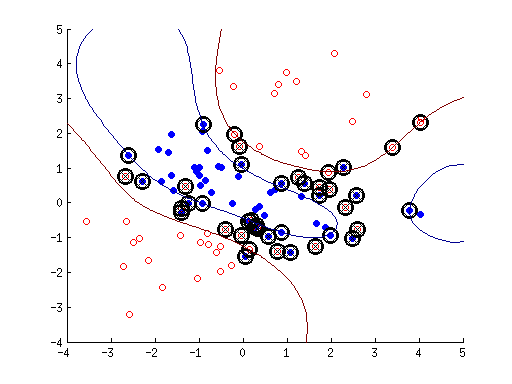
\includegraphics[width=1\textwidth]{include/graphics/nonlin_svm}
     \caption{Результат обучения нелинейной МОВ}
     \label{fig:NonLinSVM}
\end{figure}

Анализ контейнера при использовании данного метода производится в несколько этапов:
\begin{enumerate}
\item выбор характеристик стегообъектов, позволяющих судить о пустоте или заполненности контейнера и называемых \textit{признаками};
\item обучение машины опорных векторов на достаточно большой выборке пустых и заполненных стегоконтейнеров;
\item применение обученной машины для классификации.
\end{enumerate}

Конструирование пространства признаков является частным случаем задачи построения математической модели заполненного стегоконтейнера, наличие которой позволило бы легко вычислять принадлежность анализируемых объектов к тому или иному классу. Зачастую в качестве таких признаков используются статистические характеристики.

Пример, иллюстрирующий применение МОВ в задачах стегоанализа описан в работе~\cite{HistogramDFTSVM}. Авторы предлагают стегоаналитический алгоритм SHDFT:
\begin{enumerate}
\item цветной контейнер $ b $ разделяется на каналы $ b_R $, $ b_G $ и $ b_B $;
\item для каждого из них строится гистограмма частот появления значений яркости, для которой находятся математическое ожидание и дисперсия (всего 6 признаков);
\item полученные гистограммы подвергается дискретному преобразованию Фурье, для результата которого рассчитываются математическое ожидание, дисперсия, коэффициенты асимметрии и эксцесса, а также энергия сигнала во всех трёх каналах (всего 15 признаков);
\item рассчитывается математическое ожидание разности гистограммы частот яркостей и результата дискретного преобразования Фурье (всего 3 признака);
\item пункты 1-4 повторяются для всей обучающей выборки, используемой для обучения МОВ.
\end{enumerate}

Подход, демонстрирующий использование признаков из областей преобразования исходного изображения, продемонстрирован в~\cite{RishidasS2015} производится кадрирование набора изображений на фрагменты размером $ 16 \times 16 $ пикселей. Каждый фрагмент подвергается дискретному косинусному и вейвлет-преобразованиям, таким образом, в трёх областях рассчитывается математическое ожидание, дисперсия, коэффициенты асимметрии и эксцесса.

\clearpage